
\chapter{General Context}
\renewcommand{\chaptername}{Chapter}
This chapter introduces the general context of the conducted work. 
We start by presenting the hosting company, describing its line of work and enumerating its clients. Afterwards, we proceed by relating the goal of our project as well as the expected results.

\section {Presentation of the hosting company}

Through this section, we present the hosting company and enlist the different phases of its evolution.

\subsection{ATHENA Experts}

%We define different terms and clarify various concepts about the company. As a matter of fact, WebForge delivers SaaS product in association with Classnco. The product is called YusoFleet, and each client uses this solution according to his preferences.  
ATHENA is a service company specialized in Information Security and governance. Since 2007, ATHENA is supporting its clients in technical, operational and organizational aspects related to its specialization areas. Operating internationally, ATHENA already has 4 branches in :
\begin{itemize}
\item Paris (France)
\item Bucharest (Romania)
\item Tunis (Tunisia)
\item Kinshasa (Democratic Republic of Congo)
\end{itemize}
Driven by a growing development, ATHENA intends to strengthen its international presence in order to be closer to its clients.
%\begin{itemize}[label=\ding{217}]\item \textbf{WebForge Technologies SARL}Webforge Technologies SARL is a Tunisian startup that develops innovative solutions for urban transport. It is in fact a subsidiary company of Classnco.


%\item\textbf{Classnco}Launched in 2012, the Parisian start-up Class \& Co is developing its first stream optimization software for the transport of persons. The company designs, develops and markets software for a SAAS existing transport stakeholders on demand.It provides them with technology solutions that automate and optimize certain key business processes including booking, dynamic management of drivers schedules and other operations (reporting shopping, billing, ...).

%\item 
%\textbf{YusoFleet}

%YusoFleet is the first digital solution to facilitate the activity of radio taxis, ambulance and VTC. The main idea is to offer a unique and simple tool for scanning reservation management, as well as exchanges with customers and drivers.

%Two years after its founding, they connect today approximately 5,000 vehicles and performed almost 500,000 automatic dispatchs successfully. They equip fleets of 3 vehicles to 1000 and, for example, this software is used by leading motorcycle taxi in Paris. \cite{linkedin}



%\end{itemize}


\subsection{Provided services }

\subsubsection{PCI DSS}
ATHENA supports its clients with PCI DSS (Payment Card Industry Data Security Standard) approach and offers the following services :
\begin{itemize}
\item PCI DSS training. 
\item Supports in the scoping study and defining the scope of your PCI DSS certification project.
\item Supports in PCI DSS compliance and mainting of the certification
\item Recurrent Audits of your PCI DSS scope.
\item Mock Audit to prepare for PCI DSS certification.
\end{itemize}
\subsubsection{Audit}
ATHENA offers a comprehensive set of IT security audits, including :
\begin{itemize}
\item Infrastructure Penetration Testing.
\item Wireless Penetration Testing.
\item Application Penetration Testing.
\item Social Engineering Penetration Testing.
\item Source code security audit.
\item Technical Audit.
\item Configuration Audit.
\item Compliance Audit.
\item Recrrent Audit.
\end{itemize}
\subsubsection{Consulting}

ATHENA leverages an extensive knowledge of the IT security field to offer the following consulting services :
\begin{itemize}
\item Risk Analysis.
\item Development/review of security policies.
\item Secure architecture design.
\item Technical and technological study and advise.
\item Information Security Management System (ISMS) implementation assistance.
\item Chief Information Security Officer (CISO) assistance/coaching.
\item Project management assistance.
\end{itemize}
\subsubsection{Deployment}
Through the following services, ATHENA assists its clients in setting up and developing a secure and efficient information system that meets the ever-growing requirements of the final users while respecting compliance obligations :
\begin{itemize}
\item Design of secure solutions.
\item Deployment of secure solutions.
\item Testing of information system proper operations.
\item Technical trainings and skills transfer.
\end{itemize}
Key Solutions deployed by ATHENA :
\begin{itemize}
    \item SIEM (Security information and event management).
    \item DLP (Data Loss Prevention).
    \item Data Encryption and Digital Signature.
    \item VMS (Vulnerability Management System).
    \item Endpoint Detection and Response.
    \item Next Generation Firewalls.
    \item Digital forensics.
    \item SOC (Security Operations Center).
\end{itemize}
\begin{figure}[!htpb]
\begin{center}

\includegraphics{images/ATHENAdeployment.png}
\caption{ATHENA's deployed solutions}
\label{schema}
\end{center}
\end{figure} 
\subsubsection{Digital Forensics}
ATHENA's digital forensics team addresses potential security incidents as well as malicious cyber-attacks via the following services :
\begin{itemize}
    \item Trackback of the cyber-attack or the security incident.
    \item Collection and preservation of relevant evidence.
    \item Intruders identification.
    \item Assessment of the damage's extent.
    \item Protection against attack renewal.
\end{itemize}
\begin{figure}[!htpb]
\begin{center}

\includegraphics{images/ATHENAdigitalf.png}
\caption{Encase's Logo}
\label{schema}
\end{center}
\end{figure} 
\subsubsection{Managed Services}
Thanks to ATHENA's Security Operation Center (SOC), ATHENA remotely provides its clients with the following services:
\begin{itemize}
    \item Real time monitoring of services and equipment.
    \item Logs collection and correlation.
    \item Real time security events management.
    \item Hotline and incident management.
    \item Performances monitoring.
    \item Administration and exploitation of services and equipment.
    \item Vulnerability management.
    \item Compliance tests.
    \item Data Leak Prevention.
\end{itemize}
\subsubsection{Business Continuity / Disaster Recovery Plan}
In order to ensure the continuity / quick and efficient recovery of its clients business in case of a disaster, ATHENA offers the following services :
\begin{itemize}
    \item Development of Business Continuity Plan (BCP) and/or Disaster Recovery Plan (DRP).
    \item Implementation of the BCP and/or DRP.
    \item Evaluation of the BCP and/or DRP efficiency and adequacy with the context of the client and the enforced regulations.
    \item Optimization of the "Efficiency / Cost" rate of the BCP and DRP.
    \item Disaster simlation.
\begin{figure}[!htpb]
\begin{center}
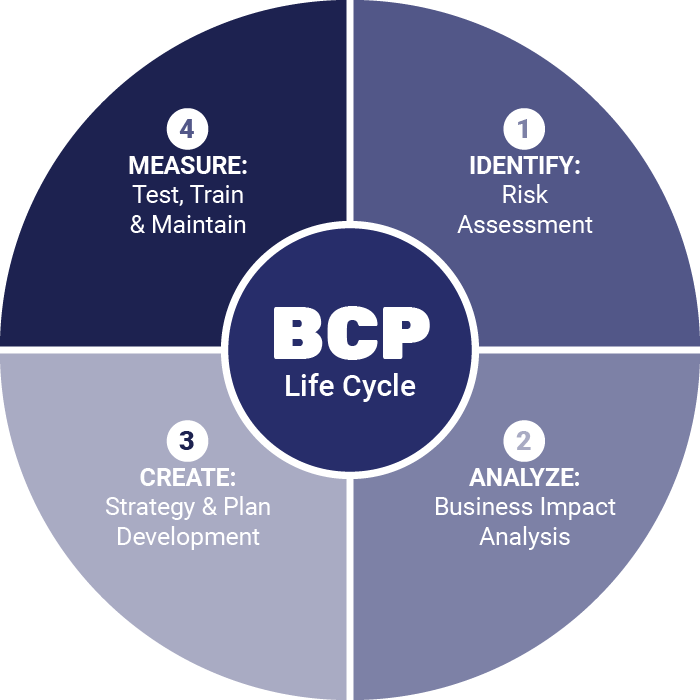
\includegraphics[ height=1.9 in]{images/ATHENABCP.png}
\caption{Business Continuity Plan}
\label{schema}
\end{center}
\end{figure} 
\end{itemize}

\subsubsection{Training and Awareness}
ATHENA offers a comprehensive range of training that cover various aspects of information security. These training courses are specifically adapted to the context, the business needs as well as the constraints of the client.
ATHENA's training covers four main areas :
\begin{figure}[!htpb]
\begin{center}

\includegraphics[ height=1 in]{images/ATHENAPECB.png}
\caption{EC-Council Logo}
\label{schema}
\end{center}
\end{figure}
\begin{itemize}
    \item Information System Security.
    \item Risk management.
    \item Information System Audit.
    \item Internal Audit.
\end{itemize}
\begin{figure}[!htpb]
\begin{center}

\includegraphics[ height=0.8 in]{images/ATHENAECCOUNCIL.png}
\caption{EC-Council Logo}
\label{schema}
\end{center}
\end{figure}
\begin{itemize}[label=\ding{50}]

\item\textit{}
ATHENA provides to its clients the design and implementation of awareness programs.
\end{itemize}
\begin{figure}[!htpb]
\begin{center}

\includegraphics[ height=0.5 in]{images/ATHENAconsicio.png}
\caption{Conscio Logo}
\label{schema}
\end{center}
\end{figure} 
\subsubsection{Governance and Strategy}
ATHENA leverages its know-how in governance and strategy to offer the following services :
\begin{itemize}
    \item IT governance diagnostic.
    \item Implementation if the IT strategy.
    \item Business Process Re-engineering.
\end{itemize}

%CONTEXT OF THE PROJECT----------------------------
\section{Context of the project}

This section includes, first, a presentation of the context of our internship, followed by a brief description of the project as well as the problem settings.

\subsection{Scope}

This project was conducted in the context of a summer internship. It is specified in the official program of the Private Superior School of Engineering and Technology (ESPRIT), as one of the requirements in order to obtain the engineering diploma. It involves a company immersion internship within four to six months during the summer. 

Our internship was held at ATHENA Experts SARL during the period from January , 2018 to July , 2018.

\subsection{Problem description} 


Once accomplishing the proof of concept, each company is struggling to maintain its fair share in the market. Especially when dealing with various clients that have put their trust and money and have invested a lot hoping to receive efficient services. As the challenge applies to ATHENA, the company is determined to provide the fastest and most powerful security services to their clients. Hence, improvements have been made over the past years but the fleet domain is so competitive that it is never enough.

Almost every company today has at least some defensive cyber security equipment like a firewall, intrusion protection, URL filtering, email filtering and antivirus. These are the right basics to secure your employees against the Wild West that is the internet.

Here’s the hard truth, you can’t stop all attempts or attacks on your enterprise. Even the greatest preventative security solution deployed on every endpoint across your corporate network, will let you down eventually. Whether it’s a threat designed to bypass traditional or next-generation threat detection systems, a zero-day attack exploiting an unknown backdoor, or a malicious insider threat, something will break through.

When that does happen, to make sure your Enterprise's data is secure, you must identify the malicious activity and its main cause so you can prevent it from spreading to other servers/services. In turn, this necessitates the constant monitoring of your enterprise's databases and logs or unusual and possibly malicious activity.

Therefore, many enterprises have established a dedicated security operation center (SOC), also placed in a distinct facility that can respond to digital incidents to evaluate and enforce your security policies.

However, placing a security operation center can be complex and critical since it can drain your enterprise's resources, staff and time seriously. Therefore, the main purpose of our project is to provide efficient and methodical features in order to enhance and develop a new version of ATHENA's SOC 

%%%%%%%%%%%%%%%%%%%%%%%%%%%%%%%%%%%%%%%%%%%%%%%%%%%%%%%%%%%%%%
\ifx

As shown in the figure, the solution offered by Classnco is a SaaS product that is deployed on the cloud. Companies who own their proper vehicle are potential clients. They approach Classnco and demand a customized software to automatically manage their fleet after paying the proper fees. They are called Saas Companies.

A SaaS company is a client that fully utilize the product. Hence, they may access the BackEnd workplace to manage and regulate profiles, vehicles, payment methods...
The users who handle the BackEnd are called SaaS offices. They are part of the SaaS company. 

Afterwards, come the front-end users. On one hand, there are the regular users that are searching for a ride. They follow an inclusive offer once they approach a SaaS company. Each company enlists its personal offers and prices. This user may eventually book rides and choose the type of the vehicle and take advantage of various features, depending on the company.

On the other hand, front-end users include also the drivers. These individuals are employees for the SaaS company, and they usually drive the vehicles of the hosting company. 
They use their own workspace of the product, as the driver's interface notifies and reminds them of booked rides. They are then geolocated in order to keep track of them.

However, their geolocation is not sufficient as the control of a large number of drivers is not practical. Furthermore, BackEnd users are not able to gather statistics from reviewing the front-end users' activities. As a further matter, SaaS office should not only observe real time activities, but also enjoy a practical and intuitive interface in order to accomplish its satisfaction.  

Therefore, the main purpose of our project is to provide efficient and methodical features for the BackEnd user.
\fi
%%%%%%%%%%%%%%%%%%%%%%%%%%%%%%%%%%%%%%%%%%%%%%%%%%%%%%%%%%%%%%%%%%
\begin{figure}[!htpb]
\begin{center}
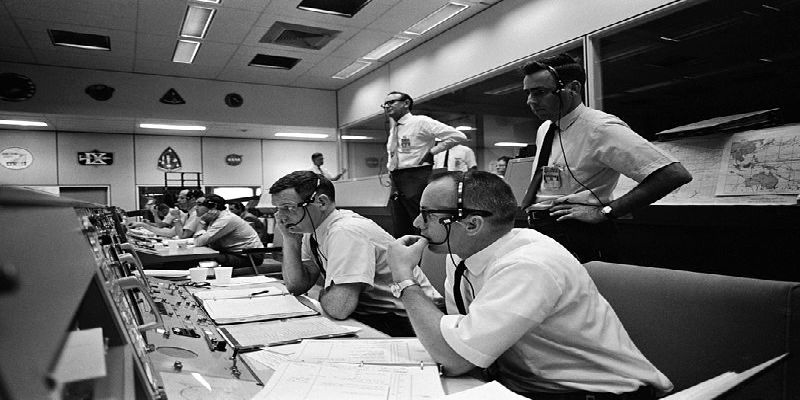
\includegraphics[height=2.0 in]{images/ATHENAsoc.jpg}
\caption{Monitoring centers }
\label{schema}
\end{center}
\end{figure} 
\section{Agile methodology: Kanban}

In this section, we introduce the working methodology adopted during the internship.
As a matter of fact, we chose to work with the agile Kanban to organize our tasks and
assignments.
\subsection{Definition}

Kanban is a lean method to manage and improve work across human systems. This
approach aims to manage work by balancing the demands with available capacity and improving the handling of system-level bottlenecks.

Work items are visualized to give participants a view of progress and process, from start
to finish usually via a Kanban board. Work is pulled as capacity permits, rather than work
being pushed into the process when requested. This provides a visual process management
system which aids decision-making about what, when and how much to produce.
\subsection{Characteristics}

The main characteristics of the adopted methodology are:
    \begin{itemize}
        \item Visualization: Creation of a board with post-it notes describing the tasks to perform
        and specifying their progress as illustrated on Figure \ref{kanban}.
        \item Limitation of the quantity of the work in progress: Split the list of tasks that would be endless into a series of reduced lists.
        \item Continuous Improvement: Ability to add new tasks whenever the capacity allows it.
    \end{itemize}
\begin{figure}[!htpb]
\begin{center}
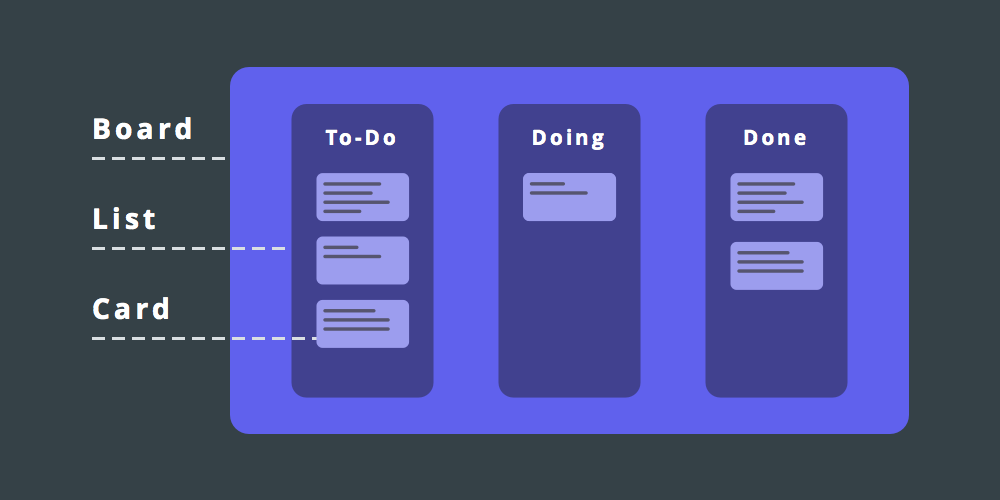
\includegraphics[height=3.0 in]{images/ATHENAkanban.png}
\caption{Illustration of a Kanban board}
\label{kanban}
\end{center}
\end{figure} 
\subsection *{Conclusion}

This chapter included a presentation of the hosting company, the context of the project and an overview of the problem settings. Moreover, we defined our agile methodology. The next chapter is devoted for the study
of the state of the art, the features that are already implemented and those that should be added in this project.